\section{The question and the coordinates}
\label{l1:setting}
\noindent\textbf{Aim.} Starting from Laurain's distributed second shape
 derivative, obtain the two eigenvalues of every Fourier block of the
 vertex Hessian. A suggested 90-minute session spends 20 minutes on vertex
 calculus, 25 on the local blocks, 30 on Fourier reduction, and 15 on the
 checks and exercises. The prerequisite is the weak Dirichlet problem and
 the meaning of a second shape derivative; no interval arithmetic is used
 in this lecture.

For a polygon $P$, let
\[
 -\Delta u=1\quad\hbox{in }P,\qquad u\in H^1_0(P),\qquad
 J(P)=\frac12\int_Pu=\frac12\int_P|\nabla u|^2.
\]
Our objective is $\F(P)=J(P)/A(P)^2$, where $A(P)=|P|$.
Conventional torsional rigidity for this PDE is $2J$. Multiplying the
objective by two changes eigenvalue magnitudes, but not their signs.
The dilation laws $u_{tP}(tx)=t^2u_P(x)$ and $J(tP)=t^4J(P)$ explain the
power $A^2$ in the denominator.

Fix the regular polygon of circumradius one. Throughout the course,
\[
 \vartheta=\frac{2\pi}{n},\qquad
 a_j=(\cos(j\vartheta),\sin(j\vartheta)),\qquad
 T_j=\operatorname{conv}\{0,a_j,a_{j+1}\}.
\]
Indices are taken modulo $n$. The same $\vartheta$ is used everywhere;
we do not give separate names to its half-angle, its multiples, or its
sine and cosine. The rotation through $j\vartheta$ is $R_j$.
The vector of vertex coordinates is interleaved as
$(x_0,y_0,x_1,y_1,\ldots)$.

\begin{center}
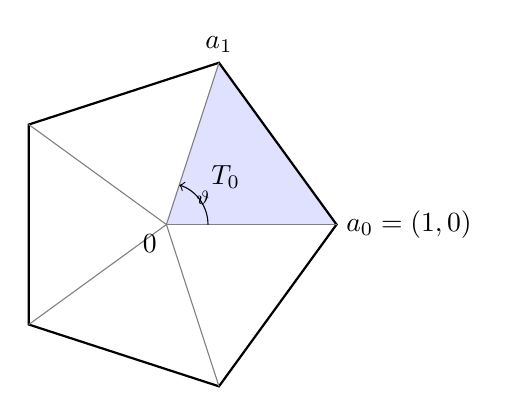
\begin{tikzpicture}[scale=1.6]
\foreach \j in {0,...,4} {\coordinate (a\j) at ({72*\j}:1.35);}
\fill[blue!12] (0,0)--(a0)--(a1)--cycle;
\draw[thick] (a0)--(a1)--(a2)--(a3)--(a4)--cycle;
\foreach \j in {0,...,4} {\draw[gray] (0,0)--(a\j);}
\node[below left] at (0,0) {$0$};
\node[right] at (a0) {$a_0=(1,0)$};
\node[above] at (a1) {$a_1$};
\node at (.47,.38) {$T_0$};
\draw[->] (.33,0) arc (0:72:.33);
\node at (.29,.21) {\scriptsize$\vartheta$};
\end{tikzpicture}
\end{center}

Let $\phi_j$ be the continuous affine hat on this coarse fan, one at
$a_j$ and zero at its other vertices, including the centre. A vertex
perturbation $q=(q_j)_{j=0}^{n-1}$, $q_j\in\R^2$, is extended into the
polygon by
\[
 \theta_q(x)=\sum_j\phi_j(x)q_j.
\]
This formula says exactly how points inside the polygon move: the map
$x\mapsto x+s\theta_q(x)$ moves the boundary vertices as prescribed and
fixes the centre. For sufficiently small $s$, it is a bi-Lipschitz map.
Its gradient is constant on each fan triangle. This last fact will be
used in every subsequent calculation.

\section{From a shape derivative to a vertex Hessian}
\label{l1:vertex}
For each vertex, $U_i=(U_i^1,U_i^2)$ collects the material derivatives of
$u$ under displacements of that vertex in the two coordinate directions.
The superscript is a component, not a derivative order. Differentiating
the pulled-back weak equation gives, for scalar $v\in H^1_0(P)$,
\begin{align}
 \int_P DU_i\nabla v={}&
 \int_P-(\nabla u\cdot\nabla v)\nabla\phi_i
 +(\nabla\phi_i\cdot\nabla v)\nabla u\notag\\
 &\quad +(\nabla\phi_i\cdot\nabla u)\nabla v+v\nabla\phi_i.
 \label{l1:material}
\end{align}
For the direction $q$, the scalar material derivative is
$u_q=\sum_iq_i\cdot U_i$. All these functions have zero Dirichlet trace
on the reference polygon: the boundary condition was pulled back before
being differentiated.

We assume Laurain's distributed formula \cite[Proposition 14]{Laurain2020}.
Its planar reduction is manuscript equation~\meq{eq:HJ}:
\begin{align}
 (D^2J)_{ij}={}&\int_P DU_iDU_j^T\notag\\
 &+\int_P\left(\tfrac12|\nabla u|^2+u\right)
 (\nabla\phi_i\otimes\nabla\phi_j-
  \nabla\phi_j\otimes\nabla\phi_i)\notag\\
 &-\int_P(\nabla\phi_i\cdot\nabla\phi_j)
              (\nabla u\otimes\nabla u).
 \label{l1:HJ}
\end{align}
This is a $2\times2$ block. For example its Gram contribution in component
$(p,q)$ is $\int_P\nabla U_i^p\cdot\nabla U_j^q$.

Here is the algebra behind the reduction. For any three planar vectors
$p,r,g$,
\begin{align*}
 &(r\cdot g)p\otimes g+(p\cdot g)g\otimes r
 -(p\cdot g)r\otimes g-(r\cdot g)g\otimes p\\
 &\hspace{25mm}=|g|^2(p\otimes r-r\otimes p).
\end{align*}
Checking the two diagonal entries gives zero on both sides; checking one
off-diagonal entry gives the other by antisymmetry. Substitute
$p=\nabla\phi_i$, $r=\nabla\phi_j$, $g=\nabla u$ in Laurain's integrand.
The remaining terms proportional to $u$ give the skew expression in
\eqref{l1:HJ}. This is a two-dimensional simplification; it should not be
used unchanged in dimension three.

There are two useful structural checks. First, individual blocks need not
be symmetric, but $(D^2J)_{ji}=((D^2J)_{ij})^T$. Second, the last two terms
are local: the hats have overlapping gradients only for identical or
neighboring vertices. The Gram term is the only generally dense part.

\subsection{The area correction must be differentiated too}
The shoelace formula gives
\[
 A=\frac12\sum_j(x_jy_{j+1}-y_jx_{j+1}),\qquad
 \nabla_{a_i}A=\frac12(y_{i+1}-y_{i-1},x_{i-1}-x_{i+1}).
\]
The only nonzero mixed second derivatives connect neighboring vertices:
$A_{x_i y_{i+1}}=1/2$ and $A_{y_i x_{i+1}}=-1/2$, together with their
symmetric counterparts. At the regular polygon,
$A=n\sin\vartheta/2$ and $\nabla_{a_i}A=\sin\vartheta\,a_i$.

By the ordinary product rule,
\begin{align}
 D^2\F={}&A^{-2}D^2J-2JA^{-3}D^2A\notag\\
 &-2A^{-3}(\nabla J\otimes\nabla A+\nabla A\otimes\nabla J)
 +6JA^{-4}\nabla A\otimes\nabla A.
 \label{l1:HFgeneral}
\end{align}
Dihedral symmetry makes $\nabla_{a_i}J$ a common multiple of $a_i$.
Euler's identity for the degree-four functional $J$ then gives
\[
 \nabla J=\frac{2J}{A}\nabla A,
 \qquad D\F(P_n)=0.
\]
Substitution into \eqref{l1:HFgeneral} yields
\begin{equation}
 D^2\F=A^{-2}D^2J-2JA^{-3}D^2A
              -2JA^{-4}\nabla A\otimes\nabla A.
 \label{l1:HF}
\end{equation}
This formula is valid at the regular polygon. On the area-tangent space,
$D^2J-(2J/A)D^2A$ has the same signs as $D^2\F$.
One must not inspect $D^2J$ alone: radial dilation increases $J$.

\section{Compute the local part on two triangles}
\label{l1:local}
The hat gradients at vertex zero are
\[
 \nabla\phi_0=(1,-\cot\vartheta)\text{ on }T_0,
 \qquad
 \nabla\phi_0=(1,\cot\vartheta)\text{ on }T_{-1},
\]
and zero elsewhere. Also,
$\nabla\phi_1=(0,1/\sin\vartheta)$ on $T_0$ and
$\nabla\phi_{-1}=(0,-1/\sin\vartheta)$ on $T_{-1}$.
These identities follow by solving the three nodal interpolation equations,
not by differentiating a trigonometric interpolant.

Only three sector integrals are needed:
\[
 X=\int_{T_0}u_x^2,\qquad Y=\int_{T_0}u_y^2,
 \qquad Z=\int_{T_0}u_xu_y.
\]
Reflection across each radial side makes $\partial_nu=0$ there.
On the polygon side $u=0$. Integration by parts within $T_0$ therefore gives
\[
 X+Y=\int_{T_0}u=\frac{2J}{n},\qquad
 \int_{T_0}(\tfrac12|\nabla u|^2+u)=\frac{3J}{n}.
\]
Reflection across the sector bisector diagonalizes the sector energy tensor
in the bisector basis. In Cartesian coordinates this means
\begin{equation}
 (Y-X)\sin\vartheta+2Z\cos\vartheta=0.
 \label{l1:sector}
\end{equation}
In particular,
$-X\sin\vartheta+Z\cos\vartheta=-J\sin\vartheta/n$.
This identity is the cancellation to remember; storing $Z$ separately is
unnecessary for the final symbol.

Write $L_j$ for the first block row of the local, non-Gram part of $D^2J$.
Substitution of the hat gradients into \eqref{l1:HJ} gives
\begin{align}
 L_0&=-\frac{2}{\sin^2\vartheta}
          \begin{pmatrix}X&0\\0&Y\end{pmatrix},\notag\\
 L_1&=\frac{\cos\vartheta}{\sin^2\vartheta}
          \begin{pmatrix}X&Z\\Z&Y\end{pmatrix}
       -\frac{3J}{n\sin\vartheta}\begin{pmatrix}0&-1\\1&0\end{pmatrix},\notag\\
 L_{-1}&=\frac{\cos\vartheta}{\sin^2\vartheta}
          \begin{pmatrix}X&-Z\\-Z&Y\end{pmatrix}
       +\frac{3J}{n\sin\vartheta}\begin{pmatrix}0&-1\\1&0\end{pmatrix}.
 \label{l1:localblocks}
\end{align}
All other $L_j$ vanish. To check the sign in $L_1$, note that
$\nabla\phi_0\cdot\nabla\phi_1=-\cos\vartheta/\sin^2\vartheta$,
whereas
$\nabla\phi_0\otimes\nabla\phi_1-
 \nabla\phi_1\otimes\nabla\phi_0$
is the negative of the displayed rotation matrix divided by
$\sin\vartheta$.

\subsection{What remains unknown in the sector integrals?}
If $\Delta_n$ denotes the difference of the energies parallel and
perpendicular to the sector bisector, rotation of that diagonal tensor gives
\[
 X=\frac Jn+\frac{\Delta_n}{2}\cos\vartheta,\quad
 Y=\frac Jn-\frac{\Delta_n}{2}\cos\vartheta,\quad
 Z=\frac{\Delta_n}{2}\sin\vartheta.
\]
Symmetry alone does not determine $\Delta_n$. The manuscript's mixed
Dirichlet--Neumann torsion problem provides an analytic characterization
of it; the fixed-mesh certificate does not need that separate computation.
For the square, $X=Y=J/4$ even though $Z$ need not vanish. The sector is
not symmetric under reflection in the Cartesian axes individually.

\section{Why radial and tangential coordinates reveal the spectrum}
\label{l1:fourier}
At vertex $j$, the radial unit vector is $a_j$ and the tangential unit
vector is $(-\sin(j\vartheta),\cos(j\vartheta))$. They are the columns
of $R_j$. With $\mathsf R=\operatorname{diag}(R_0,\ldots,R_{n-1})$, set
\[
 H=\mathsf R^TD^2\F\mathsf R.
\]
This is an orthogonal change of coordinates, so eigenvalues are unchanged.
In these coordinates rotation of the polygon merely shifts the vertex
index. Consequently $H_{ij}=C_{j-i}$, where $C_{-j}=C_j^T$.

The block-circulant reduction is due to Tee \cite{Tee2007} and is used in
this polygonal setting by Bogosel and Bucur \cite{BogoselBucur2024}.
It can be proved in one line. For a sequence
$v_j=e^{ikj\vartheta}w$, $w\in\mathbb C^2$,
\[
 (Hv)_i=\sum_j C_{j-i}e^{ikj\vartheta}w
 =e^{iki\vartheta}\left(\sum_{j=0}^{n-1}e^{ikj\vartheta}C_j\right)w.
\]
Thus the $k$th Fourier subspace carries the $2\times2$ matrix
\begin{equation}
 B_k=\sum_{j=0}^{n-1}e^{ikj\vartheta}C_j.
 \label{l1:symbol}
\end{equation}
The normalized discrete Fourier transform is unitary; the multiset of all
$2n$ Hessian eigenvalues is the union of the spectra of these $n$ blocks.

Symmetry gives $B_k^*=B_k$. Reflection in the axis through vertex zero
acts as $\operatorname{diag}(1,-1)$ on radial/tangential components and
sends $j$ to $-j$. The diagonal sequences are even and the off-diagonal
sequence is odd. Therefore
\begin{equation}
 B_k=\begin{pmatrix}\alpha_k&i\gamma_k\\-i\gamma_k&\beta_k\end{pmatrix},
 \qquad
 \mu_k^\pm=\frac{\alpha_k+\beta_k
 \pm\sqrt{(\alpha_k-\beta_k)^2+4\gamma_k^2}}2.
 \label{l1:eigenvalues}
\end{equation}
The parameters $\alpha_k,\beta_k,\gamma_k$ are real. These are manuscript
equations (\meq{eq:symbol-entries})--(\meq{eq:mode-eigs}). The sign of the imaginary
entry depends on the Fourier convention; the convention in
\eqref{l1:symbol} is fixed throughout these notes.

\subsection{The explicit cancellation with area}
The radial/tangential area symbol is
\[
 \sin\vartheta\cos(k\vartheta)I
 -i\cos\vartheta\sin(k\vartheta)
                  \begin{pmatrix}0&-1\\1&0\end{pmatrix}.
\]
In the first row, the local blocks become $L_jR_j$, since $R_0=I$.
Multiply the three matrices in \eqref{l1:localblocks} by $R_j$, use
\eqref{l1:sector}, and subtract the area contribution in \eqref{l1:HF}.
The result is
\begin{align}
 &A^{-2}\sum_{j=-1}^{1}e^{ikj\vartheta}L_jR_j
 -2JA^{-3}\left[\sin\vartheta\cos(k\vartheta)I
 -i\cos\vartheta\sin(k\vartheta)
       \begin{pmatrix}0&-1\\1&0\end{pmatrix}\right]\notag\\
 &\hspace{15mm}=-\frac{2(1-\cos(k\vartheta))}{A^2\sin^2\vartheta}
                    \begin{pmatrix}X&0\\0&Y\end{pmatrix}.
 \label{l1:cancellation}
\end{align}
The explicit off-diagonal term disappears completely. The rank-one term
$\nabla A\otimes\nabla A$ in \eqref{l1:HF} acts only on the constant
radial sequence, hence only on mode zero.

For clarity, introduce the scalar rotated components already used in the
manuscript:
\[
 U_{j,r}=\cos(j\vartheta)U_j^1+\sin(j\vartheta)U_j^2,\quad
 U_{j,t}=-\sin(j\vartheta)U_j^1+\cos(j\vartheta)U_j^2,
 \qquad a(v,w)=\int_P\nabla v\cdot\nabla w.
\]
The three genuinely nonlocal quantities are
\begin{align*}
 G^{rr}_k&=\sum_j\cos(kj\vartheta)a(U_0^1,U_{j,r}),\\
 G^{tt}_k&=\sum_j\cos(kj\vartheta)a(U_0^2,U_{j,t}),\\
 G^{rt}_k&=\sum_j\sin(kj\vartheta)a(U_0^1,U_{j,t}).
\end{align*}
For every nonzero mode, \eqref{l1:cancellation} now yields
\begin{equation}
 \boxed{\begin{aligned}
 \alpha_k&=A^{-2}\left[G^{rr}_k-
          \frac{2(1-\cos(k\vartheta))X}{\sin^2\vartheta}\right],\\
 \beta_k&=A^{-2}\left[G^{tt}_k-
          \frac{2(1-\cos(k\vartheta))Y}{\sin^2\vartheta}\right],\\
 \gamma_k&=A^{-2}G^{rt}_k.
 \end{aligned}}
 \label{l1:finalentries}
\end{equation}
These are the requested Hessian eigenvalue formulas together with
\eqref{l1:eigenvalues}. Their trace contains the explicit penalty
$-4(1-\cos(k\vartheta))J/(nA^2\sin^2\vartheta)$.
Sector anisotropy cancels from that explicit penalty; it does not cancel
from the state-dependent Gram terms.

\section{Exact zero modes and the local maximum criterion}
\label{l1:zeros}
At a critical point of a similarity-invariant function, differentiating
invariance puts the four infinitesimal similarity directions in the Hessian
kernel. The mode bookkeeping matters:
\begin{center}
\begin{tabular}{lll}\toprule
motion & radial/tangential coordinates & Fourier location\\\midrule
scaling & $(1,0)$ at every vertex & $k=0$\\
rotation & $(0,1)$ at every vertex & $k=0$\\
$x$ translation & $(\cos(j\vartheta),-\sin(j\vartheta))$ & $k=1,n-1$\\
$y$ translation & $(\sin(j\vartheta),\cos(j\vartheta))$ & $k=1,n-1$\\\bottomrule
\end{tabular}
\end{center}
Thus $B_0=0$. At $k=1$ the complex translation vector is $(1,i)$, so
$\alpha_1=\beta_1=\gamma_1$. The other eigenvalue is the trace
$\alpha_1+\beta_1$. The conjugate mode $n-1$ gives the other real
translation and the same nonzero eigenvalue.

Also $B_{n-k}=\overline{B_k}$. If $n$ is even, the Nyquist mode $k=n/2$
has zero sine sequence and $\gamma_{n/2}=0$. These are exact identities,
not quantities to be recognized by a small numerical threshold.
For a generic block, strict negativity is equivalent to
\[
 \alpha_k+\beta_k<0,\qquad \alpha_k\beta_k-\gamma_k^2>0.
\]
This determinant test excludes translation blocks, whose determinant is
exactly zero; there the trace alone is tested.

\begin{theorem}[What the numerical calculation must establish]
If every branch outside the four similarity directions is strictly
negative, the regular polygon is a strict local maximizer of $J/A^2$
modulo similarities. Equivalently, it is a strict local maximizer of $J$
at fixed area, modulo translations and rotations.
\end{theorem}
\begin{proof}
The fan pullback has smoothly parameter-dependent, uniformly elliptic
coefficients in a sufficiently small vertex neighborhood. Its inverse
solution operator is smooth, so the objective is twice differentiable.
Choose a local slice complementary to the four-dimensional similarity
orbit. The Hessian is negative definite on the slice; Taylor's theorem
gives strict decrease for small nonzero slice displacements. Every nearby
orbit meets the slice. Fixing area removes the dilation freedom.
This proves a local statement about nearby labelled polygons, not global
optimality among all polygons.
\end{proof}

\section{The quantities actually passed to the next lecture}
\label{l1:pairings}
One need not assemble the entire Hessian to evaluate its symbol. For
$1\leq k<n/2$, the following are normalized vertex displacements:
\begin{align*}
 r^c_{k,j}&=\sqrt{2/n}\cos(kj\vartheta)
                     (\cos(j\vartheta),\sin(j\vartheta)),
                     &&\text{radial, cosine},\\
 t^c_{k,j}&=\sqrt{2/n}\cos(kj\vartheta)
                     (-\sin(j\vartheta),\cos(j\vartheta)),
                     &&\text{tangential, cosine},\\
 t^s_{k,j}&=\sqrt{2/n}\sin(kj\vartheta)
                     (-\sin(j\vartheta),\cos(j\vartheta)),
                     &&\text{tangential, sine}.
\end{align*}
Their pairings give respectively
\[
 D^2\F[r_k^c,r_k^c]=\alpha_k,\quad
 D^2\F[t_k^c,t_k^c]=\beta_k,\quad
 D^2\F[r_k^c,t_k^c]=0,\quad
 D^2\F[r_k^c,t_k^s]=\gamma_k.
\]
For the Nyquist cosine directions use $(-1)^j/\sqrt n$ instead of
$\sqrt{2/n}\cos(kj\vartheta)$. The certificate encloses these real
pairings directly; it need not compute separate intervals for $X,Y,Z$
or the Gram sums.

Finally, covariance gives
\[
 U_j(x)=R_jU_0(R_j^Tx),\qquad
 U_{j,r}(x)=U_0^1(R_j^Tx),\qquad
 U_{j,t}(x)=U_0^2(R_j^Tx).
\]
The distinction between vector rotation and scalar pullback explains the
optimized code: torsion and two first-vertex PDEs supply every first
material derivative. Later second-lifting solves serve error estimation.

\subsection*{Exercises and answers for discussion}
\begin{exercise}
Derive $\nabla J=(2J/A)\nabla A$ without a boundary integral formula.
\end{exercise}
\noindent\emph{Answer.} Reflection makes each gradient radial; rotation
makes their coefficients equal. If $\nabla_{a_j}J=c a_j$, Euler's identity
gives $nc=4J$. Compare with $\nabla_{a_j}A=\sin\vartheta a_j$.

\begin{exercise}
For $n=5$, explain why the target is six negative eigenvalues, even though
there are only two representative nonzero modes.
\end{exercise}
\noindent\emph{Answer.} Modes $1,4$ contribute one physical eigenvalue each;
modes $2,3$ contribute two each. Mode zero and the two translations supply
four zeros. The total is $2+4=6$ negatives out of ten dimensions.

\begin{exercise}
Can a negative computed trace alone certify a generic $2\times2$ block?
\end{exercise}
\noindent\emph{Answer.} No. A block with eigenvalues $-2$ and $1$ has
negative trace. A determinant bound or two strictly negative eigenvalue
enclosures is also required.
